\documentclass[a11paper]{article} \usepackage{tabularx}
\usepackage{titlepage}
\usepackage{amsmath}
\usepackage{amsthm}
\usepackage{document}
\usepackage{booktabs}
\usepackage{float}
\usepackage{graphicx}
\usepackage{utils}
\usepackage{multicol}
\usepackage{subcaption}
\usepackage[dvipsnames]{xcolor}
\usepackage{enumitem}       % customizable list environments
\usepackage[toc,page]{appendix}



\title{Rapport d'APP}

\class{Éléments de statique et dynamique}
\classnb{GEN411}

\teacher{Olivier Fournier \& Rémy Rahem}

\newcommand{\todo}[1]{\begin{color}{Red}\textbf{TODO:} #1\end{color}}
\newcommand{\note}[1]{\begin{color}{Orange}\textbf{NOTE:} #1\end{color}}
\newcommand{\fixme}[1]{\begin{color}{Fuchsia}\textbf{FIXME:} #1\end{color}}
\newcommand{\question}[1]{\begin{color}{ForestGreen}\textbf{QUESTION:} #1\end{color}}

\newcommand{\dd}[1]{\frac{\partial}{\partial#1}}
\renewcommand{\vec}[1]{\overrightarrow{#1}}

\author{
  \addtolength{\tabcolsep}{-0.4em}
  \begin{tabular}{rcl} % Ajouter des auteurs au besoin
      Benjamin Chausse & -- & CHAB1704 \\
      Shawn Couture    & -- & COUS1912 \\
  \end{tabular}
}

\begin{document}
\maketitle
\tableofcontents
\newpage

\section{Analyse cinématique}
\subsection{Analyse géométrique}
\label{sec:geometry}

\noindent
\begin{minipage}[t]{0.4\textwidth}
\begin{figure}[H]
  \centering
  \begin{center}
    \includegraphics[width=\textwidth]{figures/geometry.pdf}
  \end{center}
  \caption{Tiges du bras mécanique}
  \label{fig:geometry}
\end{figure}
\end{minipage}
\hfill
\begin{minipage}[t]{0.6\textwidth}

\begin{align}
  \vec{XO} = \begin{bmatrix} 0\\l_0\\0 \end{bmatrix} \hspace{.5cm}
  \vec{OB} &= \begin{bmatrix} l_1\cos{\theta}\\ l_1\sin{\theta} \\0 \end{bmatrix} \hspace{.5cm}
  \vec{BA} = \begin{bmatrix} l_2\cos{\varphi}\\l_2\sin{\varphi} \\0 \end{bmatrix} \\
  \vec{B} = \vec{XO}+\vec{OB} &= \begin{bmatrix} l_1\cos{\theta}\\l_0+l_1\sin{\theta} \\0 \end{bmatrix} \\
  \vec{A} = \vec{B}+\vec{BA} &= \begin{bmatrix}
  l_1\cos{\theta}+l_2\cos{\varphi}\\l_0+l_1\sin{\theta}+l_2\sin{\varphi} \\0 \end{bmatrix} \\
  \intertext{Autrement dit:}
  B_x(\theta) &= l_1\cos{\theta} \\
  B_y(\theta) &= l_0+l_1\sin{\theta} \\
  \label{eq:gen-a-x}
  A_x(\theta,\varphi) &= l_1\cos{\theta}+l_2\cos{\varphi} \\
  A_y(\theta,\varphi) &= l_0+l_1\sin{\theta}+l_2\sin{\varphi} \\
\end{align}
\end{minipage}

\subsection{Vitesses}
\label{sec:speed}

Lorsque des angles fixes sont considérés, il est possible de trouver les coordonnées
$x$, $y$ en fonction de ceux-ci. Toutefois, il se peut que ces angles varient
dans le temps (essentiel à considérer pour déterminer la vitesse du
point $A$). $\theta$ et $\varphi$ sont donc dorénavant présentés comme des fonctions
pour le reste de l'analyse cinématique générale du bras mécanique :

\begin{equation*}
  \theta \rightarrow \theta(t) &\hspace{1cm} \varphi \rightarrow \varphi(t)
\end{equation*}

Déterminer la vitesse du point $A$ ne devient par la suite qu'un exercice de
dérivation dans le temps de la position, en utilisant les équations développées
à la section \ref{sec:geometry} comme fondement. Afin d'en faciliter la résolution (et
la lecture), cette opération est segmentée par composantes $x$ et $y$ dans les
sections suivantes.

\subsubsection{Composante $x$}

\begin{align}
  A_x(t) &= l_1\cos{\theta(t)}+l_2\cos{\varphi(t)} \hspace{1cm} \\
  \dd{t} A_x(t) &= \dd{t} l_1\cos(\theta(t)) + \dd{t} l_2\cos(\varphi(t)) \\
  V_A_x(t) &= \dd{t} l_1\cos(\theta(t)) + \dd{t} l_2\cos(\varphi(t)) \\
  V_A_x(t) &= l_1\dd{t} \cos(\theta(t)) + l_2\dd{t} \cos(\varphi(t)) \\
  V_A_x(t) &= l_1\left( -\sin(\theta(t))\dot\theta(t)  \right) +
    l_2\left( - \sin(\varphi(t))\dot\varphi(t) \right) \\
  V_A_x(t) &= -l_1\sin(\theta(t))\dot\theta(t)
    - l_2\sin(\varphi(t))\dot\varphi(t)
\end{align}

\subsubsection{Composante $y$}
\begin{align}
  A_y(t)&=l_0+l_1\sin(\theta(t))+l_2\sin(\varphi(t)) \\
  \dd{t}A_y(t) &=
      \dd{t}l_0
    + \dd{t}l_1\sin(\theta(t))
    + \dd{t}l_2\sin(\varphi(t)) \\
  V_{A_y}(t) &=
      \dd{t}l_1\sin(\theta(t))
    + \dd{t}l_2\sin(\varphi(t)) \\
  V_{A_y}(t) &=
      l_1\dd{t}\sin(\theta(t))
    + l_2\dd{t}\sin(\varphi(t)) \\
  V_{A_y}(t) &=
      l_1\cos(\theta(t))\cdot\dot{\theta}(t)
    + l_2\cos(\varphi(t))\cdot\dot{\varphi}(t)
\end{align}

\subsection{Accélérations}

L'accélération se définit comme étant la dérivée de la vitesse. Comme la
vitesse a déjà été définie de façon générale à la section \ref{sec:speed}, il ne suffit
qu'à en effectuer la dérivée (encore une fois par composante pour simplifier
la lecture) afin d'obtenir une solution générale de l'accélération selon
n'importe quelles fonctions décrivant le mouvement angulaire des moteurs
dans le temps.

\subsubsection{Composante $x$}

\begin{align}
  V_A_x(t) &= -l_1\sin(\theta(t))\dot\theta(t)
    - l_2\sin(\varphi(t))\dot\varphi(t) \\
  \dd{t} V_A_x(t) &= \dd{t}\left(-l_1\sin(\theta(t))\dot\theta(t)
    - l_2\sin(\varphi(t))\dot\varphi(t)\right) \\
  \alpha_A_x(t) &= -l_1 \dd{t}\sin(\theta(t))\dot\theta(t)
    - l_2\dd{t}\sin(\varphi(t))\dot\varphi(t) \\
  \alpha_A_x(t) &= -l_1 \left(
      \cos(\theta(t))\dot{\theta}(t)^2 + \sin(\theta(t))\ddot{\theta}(t)
    \right) - l_2 \left(
      \cos(\varphi(t))\dot{\varphi}(t)^2 + \sin(\varphi(t))\ddot{\varphi}(t)
    \right)
\end{align}

\subsubsection{Composante $y$}

\begin{align}
  \alpha_{A_y}(t) &=
      \dd{t} l_1\cos(\theta(t))\cdot\dot{\theta}(t)
    + \dd{t} l_2\cos(\varphi(t))\cdot\dot{\varphi}(t) \\
  \alpha_{A_y}(t) &=
      l_1\dd{t} \cos(\theta(t))\cdot\dot{\theta}(t)
    + l_2\dd{t} \cos(\varphi(t))\cdot\dot{\varphi}(t) \\
  \alpha_{A_y}(t) &=
     l_1\left(-\sin(\theta(t))\cdot\dot\theta(t)\cdot\dot{\theta}(t) + \cos(\theta(t))\cdot\ddot{\theta}(t)\right)
   + l_2\dd{t} \cos(\varphi(t))\cdot\dot{\varphi}(t) \\
  \alpha_{A_y}(t) &=
     l_1\left(\cos(\theta(t))\cdot\ddot{\theta}(t) -\sin(\theta(t))\cdot\dot\theta(t)^2 \right)
   + l_2\dd{t} \cos(\varphi(t))\cdot\dot{\varphi}(t) \\
  \alpha_{A_y}(t) &=
     l_1\left(\cos(\theta(t))\cdot\ddot{\theta}(t) -\sin(\theta(t))\cdot\dot\theta(t)^2 \right)
   + l_2\left( -\sin(\varphi(t))\cdot\dot\varphi(t)\cdot\dot{\varphi}(t) + \cos(\varphi(t))\cdot\ddot{\varphi}(t) \right) \\
  \alpha_{A_y}(t) &=
     l_1\left(\cos(\theta(t))\cdot\ddot{\theta}(t) -\sin(\theta(t))\cdot\dot\theta(t)^2 \right)
   + l_2\left(\cos(\varphi(t))\cdot\ddot{\varphi}(t) -\sin(\varphi(t))\cdot\dot\varphi(t)^2 \right)
\end{align}


\section{Cas d'études en cinématique}
\subsection{Mouvement contraint horizontalement}
\label{sec:x-bound}

\noindent
\begin{minipage}[t]{0.5\textwidth}
	\begin{figure}[H]
		\centering
		\includegraphics[width=.5\textwidth]{figures/horizontal-fig.pdf}
		\caption{$A$ contraint à un mouvement en $x$}
		\label{fig:horizontal-fig}
	\end{figure}
\end{minipage}
\begin{minipage}[t]{0.5\textwidth}
	Il est possible de déterminer un relation entre $\theta$ et $\varphi$ à l'aide
	de la figure \ref{fig:horizontal-fig}:
	\begin{align}
		% \intertext{ En supposant $\theta,\varphi \in \left[-\frac{\pi}{2},\,\frac{\pi}{2}\right]$:}
		0 &= l\sin\theta + l\sin\varphi \\
		0 &= \sin\theta  +  \sin\varphi \\
		\sin\varphi   &= -\sin\theta    \\
		\sin\varphi   &=  \sin(-\theta) \\
		% \intertext{$\arcsin$ peut être effectué de part et d'autre:}
		\varphi   &= -\theta
	\end{align}
\end{minipage} \vspace{.3cm}



Ainsi, puisque dans ce cas d'étude spécifique, $\varphi = -\theta$, les
solutions trouvées en \ref{sec:geometry} peuvent être transformées comme suit:

\begin{align}
  A_x(\theta,\varphi) = l_1\cos{\theta}+l_2\cos{\varphi} &\Rightarrow
  A_x(\theta)         = l_1\cos{\theta}+l_2\cos(-\theta)
\end{align}

Avec peu, d'effort, ce même type de transformation peut être fait pour les
équation de vitesses et d'accélération où $\theta$ dépend du temps.
Puisque $-1$ est un constante, la dérivation est triviale:

\begin{equation}
  \varphi(t)        = -\theta(t) \Rightarrow
  \dot{\varphi}(t)  = -\dot{\theta}(t)  \Rightarrow
  \ddot{\varphi}(t) = -\ddot{\theta}(t)
\end{equation}

Cela permet d'exprimer les équation de vitesse et d'accélération de $A$ comme
suit:

\begin{align}
  V_A_x(t) &= -l_1\sin(\theta(t))\dot\theta(t)
    + l_2\sin(-\theta(t))\dot\theta(t) \\
  \alpha_A_x(t) &= -l_1 \left(
      \cos(\theta(t))\dot{\theta}(t)^2 + \sin(\theta(t))\ddot{\theta}(t)
    \right) - l_2 \left(
      -\cos(-\theta(t))\dot{\theta}(t)^2 - \sin(-\theta(t))\ddot{\theta}(t)
    \right)
\end{align}

Dans le câdre de cette analyse, il est demandé de modéliser le bras entre
$\theta=0$ et $\theta=\frac{\pi}{3}$ posant que la vitesse angulaire de
$\theta$ est constante et vaut $\omega$. Puisque $\dot{\theta}(t)$ est en soit
une accélération angulaire, nous obtenons ceci:

\begin{equation}
  \dot{\theta}(t) = \omega \Rightarrow
    \ddot{\theta}(t) = 0 \Rightarrow
		\label{eq:simple-derivatives}
    \theta(t) = \omega t \\
\end{equation}

\begin{align}
	A_x(t)   &= l_1\cos(\theta(t))+l_2\cos(-\theta(t)) \Rightarrow
	A_x(t)   = l_1\cos(\omega t)+l_2\cos(-\omega t) \\
  V_A_x(t) &= -l_1\sin(\omega t)\omega
    + l_2\sin(-\omega t)\omega \\
  \alpha_A_x(t) &= -l_1 \left( \cos(\omega t )\omega^2 + \sin(\omega t )\cdot 0 \right)
    - l_2 \left( \cos(-\omega t)\omega^2 + \sin(-\omega t )\cdot 0 \right) \\
    &=
    - l_1 \cos(\omega t )\omega^2
    - l_2 \cos(-\omega t)\omega^2
\end{align}

\newpage
Toutefois l'analyse de ce cas porte sur les valeurs de
position/vitesse/accélérations selon $\theta$ et non pas selon $t$.
Les deux étant interdépendants les équation ci-dessus peuvent être mises
selon $\theta$ puisque $\theta = \omega t$ implique que:

\begin{equation}
	\label{eq:substitute-time}
	t = \frac{\theta}{\omega}
\end{equation}
Ainsi:

\begin{align}
	A_x(\theta)&= l_1\cos(\omega \frac{\theta}{\omega})+l_2\cos(-\omega \frac{\theta}{\omega}) \\
	           &= l\cos(\theta)+l\cos(-\theta) \\
						 &= l\left[\cos(\theta)+\cos(-\theta)\right] \\
  V_A_x(\theta) &= -l_1\sin(\omega \frac{\theta}{\omega})\omega
    + l_2\sin(-\omega \frac{\theta}{\omega})\omega \\
		&= -l\sin(\theta)\omega + l\sin(-\theta)\omega \\
		&= -l\sin(\theta)\omega - l\sin(\theta)\omega \\
		&= -2l\sin(\theta)\omega \\
  \alpha_A_x(\theta) &=
    - l_1 \cos(\omega \frac{\theta}{\omega} )\omega^2
    + l_2 \cos(-\omega \frac{\theta}{\omega})\omega^2 \\
    &=
    - l \cos(\theta)\omega^2
    - l \cos(-\theta)\omega^2 \\
		&= -l\omega^2 \left[ \cos(\theta) + \cos(-\theta) \right] \\
		&= -l\omega^2 \left[ \cos(\theta) + \cos(\theta) \right] \\
		&= -2l\omega^2 \cos(\theta)
\end{align}

Pour le cas à l'étude $0\leq\theta\leq\frac{\pi}{3}$, une modélisation des
équation ci-dessus peut être consulté en annexe (Figure \ref{fig:x-bound}).


\subsection{Mouvement contraint verticalement}

Dans ce cas de figure, la position en $x$ du point $A$ est définie comme étant
toujours à une distance $l$ de l'origine. D'ailleurs $l$ correspond aussi à la
longueur de $l_1$ et $l_2$. L'équation générale de $A_x$ peut être utilisé pour
contraindre $\varphi$ en fonction de $\theta$:

\begin{align}
  A_x = l_1\cos{\theta}+l_2\cos{\varphi} \Rightarrow
  l &= l\cos{\theta}+l\cos{\varphi} \\
  \label{eq:vert-simple-x}
  1 &= \cos{\theta}+\cos{\varphi} \\
  1-\cos{\theta} &= \cos{\varphi} \\
  \varphi &= \arccos(1-\cos{\theta})
\end{align}

\newpage
Pour éviter d'avoir à dériver $\varphi$ dans le temps, il est possible
d'utiliser l'équation \ref{eq:vert-simple-x} et les dérivées partielles:

\begin{align}
  1 &= \cos{\theta}+\cos{\varphi} \\
  \dd{t} 1 &= \dd{t}\left(\cos{\theta}+\cos{\varphi}\right) \\
         0 &= \dd{t}\cos{\theta}+\dd{t}\cos{\varphi} \\
         0 &= -\sin(\theta)\dot{\theta}+\dd{t}\cos{\varphi} \\
         0 &= -\sin(\theta)\dot{\theta}-\sin(\varphi)\dot{\varphi} \\
         \sin(\varphi)\dot{\varphi} &= -\sin(\theta)\dot{\theta} \\
         \dot{\varphi} &= -\frac{\sin(\theta)}{\sin(\varphi)}\dot{\theta}
\end{align}

Enfin puisque le mouvement est contraint, par définition, à un mouvement que sur
l'axe des $y$, il est seulement nécessaire d'analyser la position et la vitesse
selon cet axe. Encore une fois, les équation générales sont utilisées comme
point de départ:

\begin{align}
	A_y(t) &= l+l\sin{\theta(t)}+l\sin{\varphi(t)} \\
         &= l+l\sin{\theta(t)}+l\sin{\arccos(1-\cos(\theta(t)))} \\
         &= l+l\sin{\theta(t)}+l\sin{\arccos(1-\cos(\theta(t)))} \\
				 &= l\left[1+\sin{\theta(t)}+\sin{\arccos(1-\cos(\theta(t)))}\right] \\
  V_{A_y}(t) &=
      l_1\cos(\theta(t))\dot{\theta}(t)
    + l_2\cos(\varphi(t))\dot{\varphi}(t) \\
             &=
    l\cos(\theta(t))\cdot\dot{\theta}(t) +
    l\cos(\varphi(t))\left(-\frac{\sin(\theta(t))}{\sin(\varphi(t))}\dot{\theta}(t)\right) \\
             &=
      l\cos(\theta(t))\cdot\dot{\theta}(t)
    - l\cos(\arccos(1-\cos(\theta(t)))) \left(
        \frac{\sin(\theta(t))}{\sin(\arccos(1-\cos(\theta(t))))}\dot{\theta}(t)
      \right) \\
\end{align}

Puisque la vitesse angulaire de $\theta$ est constant est la même que dans le
cas d'étude horizontal, il est possible d'utiliser la relation de l'équation
\ref{eq:simple-derivatives} pour éliminer tout $\dot{\theta}(t)$ et
enfin tout considérer en fonction de $\theta$ au lieu du temps à l'aide de
l'équation \ref{eq:substitute-time}:

\begin{align}
	A_y(t)     &= l\left[1+\sin(\omega t)+\sin(\arccos(1-\cos(\omega t)))\right] \\
	A_y(\theta)&= l\left[1+\sin(\omega t)+\sin(\arccos(1-\cos(\omega t)))\right] \\
	           &= l\left[1+\sin(\omega \frac{\theta}{\omega})+\sin(\arccos(1-\cos(\omega \frac{\theta}{\omega})))\right] \\
	           &= l\left[1+\sin(\theta)+\sin(\arccos(1-\cos(\theta)))\right]
\end{align}
\begin{align}
  V_{A_y}(t) &=
      l\cos(\omega t)\omega
    - l\cos(\arccos(1-\cos(\omega t))) \left(
        \frac{\sin(\omega t)}{\sin(\arccos(1-\cos(\omega t)))}\omega
      \right) \\
  V_{A_y}(\theta) &=
			l\cos(\omega \frac{\theta}{\omega})\omega
		- l\cos(\arccos(1-\cos(\omega \frac{\theta}{\omega}))) \left(
				\frac{\sin(\omega \frac{\theta}{\omega})}{\sin(\arccos(1-\cos(\omega
				\frac{\theta}{\omega})))}\omega
      \right) \\
                  &=
			l\cos(\theta)\omega
		- l\cos(\arccos(1-\cos\theta)) \left(
				\frac{\sin\theta}{\sin(\arccos(1-\cos\theta))}\omega
      \right) \\
                  &=
			l\cos(\theta)\omega
		- l\cos(\arccos(1-\cos\theta)) \left(
				\frac{\sin\theta}{\sin(\arccos(1-\cos\theta))}\omega
      \right) \\
                  &=
			l\left[\cos(\theta)\omega
		- \cos(\arccos(1-\cos\theta)) \left(
				\frac{\sin\theta}{\sin(\arccos(1-\cos\theta))}\omega
			\right)\right]
\end{align}

Pour le cas à l'étude $0\leq\theta\leq\frac{\pi}{3}$, une modélisation des
équations (figure \ref{fig:vertical-plots}) avec les valeurs spécifiés au tableau
\ref{tab:values-cinematique} peut être trouvée en annexe. Aussi, les
positions de départ et de fin du bras pour cette modélisation peuvent être
consulté à la figure \ref{fig:vertical-fig}.



\section{Analyse statique}

Dans un premier temps, il est demandé d'observer la force et le moment en
$B$ alors que le bras est immobile (statique) selon l'angle auquel il se
trouve. Un DSL n'analysant que le segment $\overline{BA}$ est utilisé pour
faire abstraction de ce qui se produit en ce qui concerne $\overline{OB}$ et
de ses forces, considérant le tout commes des forces/moments externes
nécessaires à garder la tige observée immobile.

\begin{multicols}{2}
  \begin{figure}[H]
    \centering
    \includegraphics[width=0.65\linewidth]{figures/static.pdf}
    \caption{DCL de la tige $\overline{BA}$}
    \label{fig:dcl}
  \end{figure}

  \columnbreak

	\begin{definitions}[]
    \vec{\alpha_g} & Accélération gravitationelle \\
    m_A            & Masse de l'objet accroché au point $A$ \\
    m_{BA}         & Masse de la tige $\overline{BA}$ \\
    \vec{P_l_2}    & Poids de la tige $l_2$ \\
    \vec{P_A}      & Poids de l'objet accroché au point $A$ \\
    \vec{P_B}      & Poids du moteur $B$ \\
    \vec{F_B}      & Force en $B$ nécessaire afin que la somme des forces soit nulle \\
    \vec{BA}       & Tige $\overline{BA}$ \\
    \vec{BA}/2     & Moitié de la tige $\overline{BA}$ \\
    \vec{M_l_2}    & Moment au point $B$ causé par $\vec{P_l_2}$ \\
    \vec{M_A}      & Moment au point $B$ causé par $\vec{P_A}$ \\
    \vec{M_B}      & Moment en $B$ nécessaire afin que la somme des moments nul
  \end{definitions}
\end{multicols}

\begin{align}
  \vec{P_l_2} &= m_{BA} \cdot \vec{\alpha_g}
    = -9.81m_{BA}\vec{j} \\
  \vec{P_A} &= m_A \cdot \vec{\alpha_g}
    = -9.81m_A\vec{j} \\
  \vec{P_B} &= m_B \cdot \vec{\alpha_g}
    = -9.81m_B\vec{j} \\
    \sum{\vec{F}} &= \vec{P_l_2} + \vec{P_A} + \vec{F_B} + \vec{P_B}= \vec{0} \\
  \vec{0} &= -9.81m_{BA}\vec{j} + (-9.81m_A\vec{j}) + \vec{F_B} + (-9.81m_B\vec{j}) \\
  \vec{F_B} &= 9.81m_{BA}\vec{j} + 9.81m_A\vec{j} + 9.81m_B\vec{j} \\
  \vec{F_B} &= 9.81(m_{BA}+m_A+m_B)\vec{j}
\end{align}

Les moments sont calculés en fonction du point $O$. Le moment causé par le poids
du moteur n'est pas considéré puisqu'il est nul (il est à une distance 0 du
point $O$).

\begin{align}
  \vec{BA}   &= \begin{bmatrix} l_2\cos(\varphi)\\ l_2\sin(\varphi)\\ 0 \end{bmatrix} \\
  \vec{BA}/2 &= \frac{1}{2} \begin{bmatrix} l_2\cos(\varphi)\\ l_2\sin(\varphi)\\ 0 \end{bmatrix}
    = \begin{bmatrix} l_2\cos(\varphi)/2 \\ l_2\sin(\varphi)/2 \\ 0 \end{bmatrix} \\
  \vec{M_A} &= \vec{BA}\times\vec{P_A}
    = \begin{bmatrix} l_2\cos(\varphi)\\ l_2\sin(\varphi)\\ 0 \end{bmatrix}
      \times (-9.81 m_A\vec{j}) \\
    &=  \vec{i} \begin{vmatrix} l_2\sin(\varphi) & 0         \\ -9.81m_A & 0        \end{vmatrix}
      - \vec{j} \begin{vmatrix} l_2\cos(\varphi) & 0         \\ 0        & 0        \end{vmatrix}
      + \vec{k} \begin{vmatrix} l_2\cos(\varphi) & l_2\sin(\varphi) \\ 0        & -9.81m_A \end{vmatrix} \\
    &= 0\vec{i} - 0\vec{j} + \left(-9.81m_Al_2\cos(\varphi)-0\right)\vec{k}
      = -9.81m_Al_2\cos(\varphi)\vec{k} \\
  \vec{M_l_2} &= (\vec{BA}/2)\times\vec{P_l_2}
    = \begin{bmatrix} l_2\cos(\varphi)/2 \\ l_2\sin(\varphi)/2\\ 0 \end{bmatrix}
      \times (-9.81 m_{BA}\vec{j}) \\
    &=  \vec{i} \begin{vmatrix} l_2\sin(\varphi)/2 & 0           \\ -9.81m_{BA} & 0          \end{vmatrix}
      - \vec{j} \begin{vmatrix} l_2\cos(\varphi)/2 & 0           \\ 0          & 0          \end{vmatrix}
      + \vec{k} \begin{vmatrix} l_2\cos(\varphi)/2 & l_2\sin(\varphi)/2 \\ 0          & -9.81m_{BA} \end{vmatrix} \\
    &= 0\vec{i} - 0\vec{j} + \frac{-9.81m_{BA}l_2\cos(\varphi)}{2}\vec{k}
      = -\frac{9.81m_{BA}l_2\cos(\varphi)}{2}\vec{k}
\end{align}
\begin{align}
  \sum{\vec{M}} &= \vec{M_A} + \vec{M_l_2} + \vec{M_B} = \vec{0} \\
  \vec{0} &= -9.81m_Al_2\cos(\varphi)\vec{k} + \left(-\frac{9.81m_{BA}l_2\cos(\varphi)}{2}\vec{k}\right) + \vec{M_B} \\
  \vec{M_B} &= 9.81m_Al_2\cos(\varphi)\vec{k} + \frac{9.81m_{BA}l_2\cos(\varphi)}{2}\vec{k} \\
    &= 9.81\cos(\varphi)l_2(m_A+m_{BA}/2)\vec{k}
\end{align}

Pour le cas statique, l'analyse porte sur l'évolution du couple résultant $M_{B_z}$ en fonction de l'angle $\varphi$ lorsque $\varphi$ varie entre $-\frac{\pi}{3}$ et $\frac{\pi}{3}$. La modélisation présentée à la figure \ref{fig:static-torque} utilise les valeurs spécifiées au tableau \ref{tab:values-statique-dynamique}. Dans ce cas, seules les forces gravitationnelles sont considérées, l'accélération angulaire étant nulle ($\ddot{\varphi} = 0$).



\section{Analyse dynamique}

\subsection{Force \vec F_B}

En dynamique, la somme des force externes c'est

\begin{equation*}
\sum\vec F_e=m\cdot\vec\gamma_G
\end{equation*}

Hors, l'équation de la statique se transforme lorsqu'on veut trouvé $\vec F_B$ car la somme n'est plus égal à $0$:

\begin{equation*}
m\cdot\vec\gamma_G=
\vec F_B +
\begin{bmatrix}
0 \\
g\cdot(m_B+m_{BA}+m_{A}) \\
0
\end{bmatrix}
\end{equation*}

L'équation avec $\vec F_B$ isolé est:

\begin{equation*}
\vec F_B =
m\cdot\vec\gamma_G-
\begin{bmatrix}
0 \\
g\cdot(m_B+m_{BA}+m_{A}) \\
0
\end{bmatrix}
\end{equation*}

De l'équation plus haut, $\vec\gamma_G$ c'est l'accélération linéaire du centre de masse. $m$ c'est la masse total.
$\vec\gamma_G$ est exprimé par une accélération tangentielle et une accélération centripète:


\begin{equation*}
\vec\gamma_G=\vec\gamma_G^t+\vec\gamma_G^n
\end{equation*}

Ou:
	- l'accélération tangentielle c'est $\alpha\times\vec r$
	- l'accélération centripète c'est $\vec\omega\times(\vec\omega\times\vec r)$
$\vec r$ est en réalité $\vec r_{B/G}$ qui est ceci:

\begin{align}
\vec r=\frac{l_2}{2}
\begin{bmatrix}
\cos\varphi \\
\sin\varphi \\
0 \\
\end{bmatrix}

\vec r=
\begin{bmatrix}
\frac{l_2}{2}\cdot\cos\varphi \\
\frac{l_2}{2}\cdot\sin\varphi \\
0 \\
\end{bmatrix}
\end{align}

L'accélération est une constante, posé par la problématique. Et afin de simplifé les équations,
La vitesse initial est posé comme nulle: $\vec\omega=\vec0$. Ceci simplifie grandement l'équation.
Une fois remplacé, on obtient:

\begin{align}
\vec\gamma_G=\vec\gamma_G^t+\vec\gamma_G^n


\vec\gamma_G=\alpha\times\vec r+\vec\omega\times(\vec\omega\times\vec r)

\vec\gamma_G=
\begin{bmatrix}
0\\
0\\
\alpha_{AB}
\end{bmatrix}
\times
\begin{bmatrix}
\frac{l_2}{2}\cdot\cos\varphi \\
\frac{l_2}{2}\cdot\sin\varphi \\
0 \\
\end{bmatrix}
+
\vec0\times(\vec0\times\vec r)


\vec\gamma_{G_x}=0\cdot0+\alpha_{AB}\cdot\frac{l_2}{2}\cdot\sin\varphi


\vec\gamma_{G_y}=\alpha_{AB}\cdot\frac{l_2}{2}\cdot\cos\varphi - 0\cdot0


\vec\gamma_{G_z}=0\cdot\frac{l_2}{2}\cdot\sin\varphi +0\cdot\frac{l_2}{2}\cdot\cos\varphi


\vec\gamma_{G}=
\begin{bmatrix}
\alpha_{AB}\cdot\frac{l_2}{2}\cdot\sin\varphi \\
\alpha_{AB}\cdot\frac{l_2}{2}\cdot\cos\varphi \\
0
\end{bmatrix}
\end{align}
Ça se remplace facilement dans l'équation initial. Afin de rendre l'équation plus facile à lire; $m_t=m_B+m_{BA}+m_A$.
\begin{align}
\vec F_B =
m_{total}\cdot\vec\gamma_G-
\begin{bmatrix}
0 \\
g\cdot(m_B+m_{BA}+m_{A}) \\
0
\end{bmatrix}

\vec F_B =
m_{t}\cdot
\begin{bmatrix}
\alpha_{AB}\cdot\frac{l_2}{2}\cdot\sin\varphi \\
\alpha_{AB}\cdot\frac{l_2}{2}\cdot\cos\varphi \\
0
\end{bmatrix}
-
\begin{bmatrix}
0 \\
g\cdot m_t \\
0
\end{bmatrix}

\vec F_B =
\begin{bmatrix}
\alpha_{AB}\cdot m_t\frac{l_2}{2}\cdot\cos\varphi \\
\alpha_{AB}\cdot m_t\frac{l_2}{2}\cdot\sin\varphi \\
0 \\
\end{bmatrix}
-
\begin{bmatrix}
0 \\
g\cdot m_t \\
0
\end{bmatrix}

\vec F_B =
\begin{bmatrix}
\alpha_{AB}\cdot m_t\frac{l_2}{2}\cdot\cos\varphi-0 \\
\alpha_{AB}\cdot m_t\frac{l_2}{2}\cdot\sin\varphi-g\cdot m_t \\
0-0 \\
\end{bmatrix}

\vec F_B =
\begin{bmatrix}
\alpha_{AB}\cdot m_t\frac{l_2}{2}\cdot\cos\varphi \\
(\alpha_{AB}\cdot m_t\frac{l_2}{2}\cdot\sin\varphi)-g\cdot m_t \\
0 \\
\end{bmatrix}
\end{align}


\newpage
\appendix
\section{Cinématique}

\begin{table}[H]
	\centering
	\caption{Valeurs des divers termes pour les cas d'étude cinématiques}
	\label{tab:values-cinematique}
	\begin{tabular}{ll}
		\toprule
	  Variable & Valeur \\
		\midrule
		$l_0$ & 50 cm \\
		$l_1$ & 25 cm \\
		$l_2$ & 25 cm \\
		$\omega$ & 25 rad$/\textrm{s}^2$ \\
		\bottomrule
	\end{tabular}
\end{table}

\subsection{Mouvement horizontal}
\begin{figure}[H]
  \centering
	\begin{subfigure}{.45\linewidth}
		\centering
		\includegraphics[width=\textwidth]{figures/horizontal-pos.pdf}
		\caption{Position en $x$}
		\label{fig:horizontal-pos}
	\end{subfigure}
	\begin{subfigure}{.45\linewidth}
		\centering
		\includegraphics[width=\textwidth]{figures/horizontal-v.pdf}
		\caption{Vitesse en $x$}
		\label{fig:horizontal-v}
	\end{subfigure}

	\begin{subfigure}{.5\linewidth}
		\centering
		\includegraphics[width=\textwidth]{figures/horizontal-alpha.pdf}
		\caption{Accélération en $x$}
		\label{fig:horizontal-alpha}
	\end{subfigure}

	\caption{Attributs du point $A$ lorsque contraint à un mouvement horizontal}
	\label{fig:horizontal-plots}
\end{figure}

\begin{figure}[H]
  \centering
\begin{subfigure}{.26\linewidth}
		\centering
		\includegraphics[width=\textwidth]{figures/x-bound-fig-before.pdf}
		\caption{lorsque $\theta=0$}
		\label{fig:horizontal-before}
	\end{subfigure}
	\hspace{1cm}
	\begin{subfigure}{.2\linewidth}
		\centering
		\includegraphics[width=\textwidth]{figures/x-bound-fig-after.pdf}
		\caption{lorsque $\theta=\frac{\pi}{3}$}
		\label{fig:horizontal-after}
	\end{subfigure}
		\caption{Positionnement du bras contraint à un mouvement en $x$ selon $\theta$}
	\label{fig:horizontal-fig}
\end{figure}

\subsection{Mouvement vertical}

\begin{figure}[H]
  \centering
	\begin{subfigure}{.43\linewidth}
		\centering
		\includegraphics[width=\textwidth]{figures/vertical-pos.pdf}
		\caption{Position en $y$}
		\label{fig:vertical-pos}
	\end{subfigure}
	\begin{subfigure}{.43\linewidth}
		\centering
		\includegraphics[width=\textwidth]{figures/vertical-v.pdf}
		\caption{Vitesse en $y$}
		\label{fig:vertical-v}
	\end{subfigure}

	\caption{Attributs du point $A$ lorsque contraint à un mouvement horizontal}
	\label{fig:vertical-plots}
\end{figure}

\begin{figure}[H]
  \centering
	\begin{subfigure}{.36\linewidth}
		\centering
		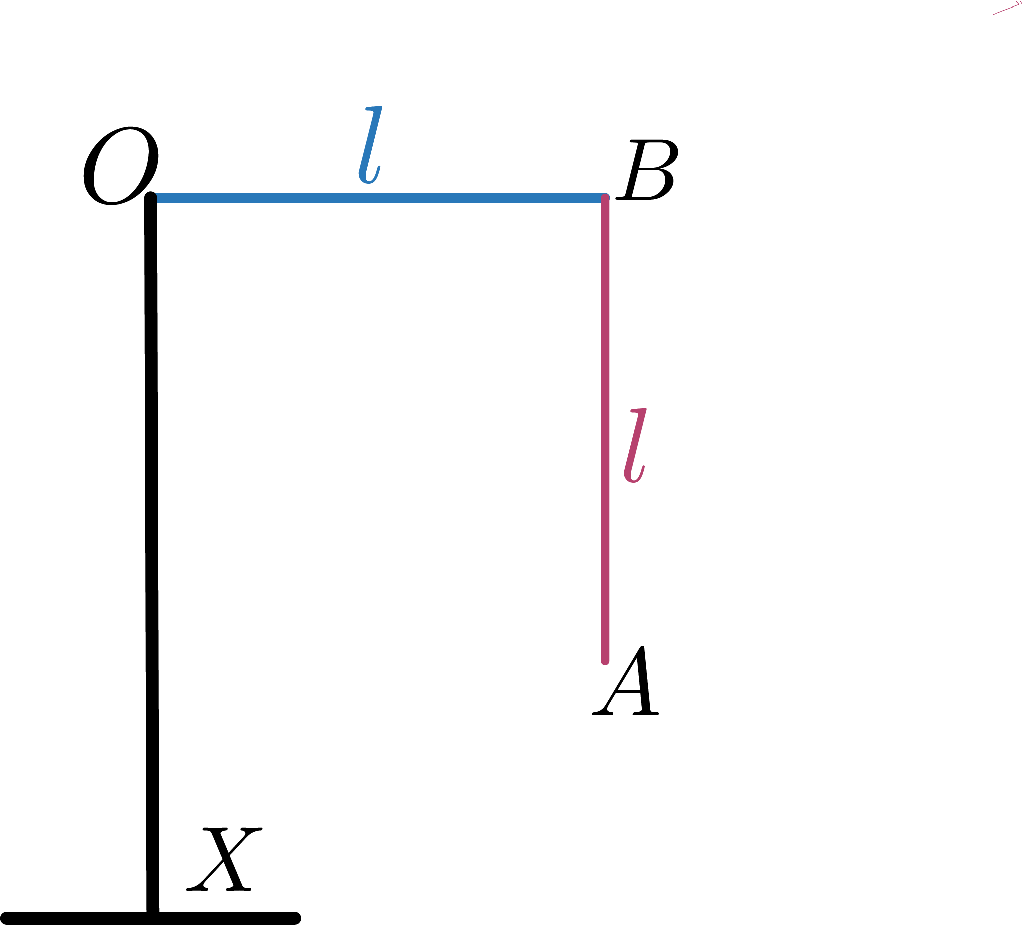
\includegraphics[width=\textwidth]{figures/vert-before.pdf}
		\caption{lorsque $\theta=0$}
		\label{fig:vertical-before}
	\end{subfigure}
	\hspace{1cm}
	\begin{subfigure}{.3\linewidth}
		\centering
		\includegraphics[width=\textwidth]{figures/vert-after.pdf}
		\caption{lorsque $\theta=\frac{\pi}{3}$}
		\label{fig:vertical-after}
	\end{subfigure}
		\caption{Positionnement du bras contraint à un mouvement en $y$ selon $\theta$}
	\label{fig:vertical-fig}
\end{figure}

\section{Simulations statiques et dynamiques}

\begin{figure}[H]
  \centering
  \includegraphics[width=0.7\textwidth]{figures/static-torque.pdf}
  \caption{Couple résultant $M_{B_z}$ en fonction de l'angle $\varphi$ (cas statique)}
  \label{fig:static-torque}
\end{figure}

\todo{Dynamique: Plot $C_b$ selon $\varphi$}

\end{document}
